% Options for packages loaded elsewhere
\PassOptionsToPackage{unicode}{hyperref}
\PassOptionsToPackage{hyphens}{url}
\PassOptionsToPackage{dvipsnames,svgnames,x11names}{xcolor}
%
\documentclass[
]{agujournal2019}

\usepackage{amsmath,amssymb}
\usepackage{iftex}
\ifPDFTeX
  \usepackage[T1]{fontenc}
  \usepackage[utf8]{inputenc}
  \usepackage{textcomp} % provide euro and other symbols
\else % if luatex or xetex
  \usepackage{unicode-math}
  \defaultfontfeatures{Scale=MatchLowercase}
  \defaultfontfeatures[\rmfamily]{Ligatures=TeX,Scale=1}
\fi
\usepackage{lmodern}
\ifPDFTeX\else  
    % xetex/luatex font selection
\fi
% Use upquote if available, for straight quotes in verbatim environments
\IfFileExists{upquote.sty}{\usepackage{upquote}}{}
\IfFileExists{microtype.sty}{% use microtype if available
  \usepackage[]{microtype}
  \UseMicrotypeSet[protrusion]{basicmath} % disable protrusion for tt fonts
}{}
\makeatletter
\@ifundefined{KOMAClassName}{% if non-KOMA class
  \IfFileExists{parskip.sty}{%
    \usepackage{parskip}
  }{% else
    \setlength{\parindent}{0pt}
    \setlength{\parskip}{6pt plus 2pt minus 1pt}}
}{% if KOMA class
  \KOMAoptions{parskip=half}}
\makeatother
\usepackage{xcolor}
\setlength{\emergencystretch}{3em} % prevent overfull lines
\setcounter{secnumdepth}{5}
% Make \paragraph and \subparagraph free-standing
\ifx\paragraph\undefined\else
  \let\oldparagraph\paragraph
  \renewcommand{\paragraph}[1]{\oldparagraph{#1}\mbox{}}
\fi
\ifx\subparagraph\undefined\else
  \let\oldsubparagraph\subparagraph
  \renewcommand{\subparagraph}[1]{\oldsubparagraph{#1}\mbox{}}
\fi


\providecommand{\tightlist}{%
  \setlength{\itemsep}{0pt}\setlength{\parskip}{0pt}}\usepackage{longtable,booktabs,array}
\usepackage{calc} % for calculating minipage widths
% Correct order of tables after \paragraph or \subparagraph
\usepackage{etoolbox}
\makeatletter
\patchcmd\longtable{\par}{\if@noskipsec\mbox{}\fi\par}{}{}
\makeatother
% Allow footnotes in longtable head/foot
\IfFileExists{footnotehyper.sty}{\usepackage{footnotehyper}}{\usepackage{footnote}}
\makesavenoteenv{longtable}
\usepackage{graphicx}
\makeatletter
\def\maxwidth{\ifdim\Gin@nat@width>\linewidth\linewidth\else\Gin@nat@width\fi}
\def\maxheight{\ifdim\Gin@nat@height>\textheight\textheight\else\Gin@nat@height\fi}
\makeatother
% Scale images if necessary, so that they will not overflow the page
% margins by default, and it is still possible to overwrite the defaults
% using explicit options in \includegraphics[width, height, ...]{}
\setkeys{Gin}{width=\maxwidth,height=\maxheight,keepaspectratio}
% Set default figure placement to htbp
\makeatletter
\def\fps@figure{htbp}
\makeatother
% definitions for citeproc citations
\NewDocumentCommand\citeproctext{}{}
\NewDocumentCommand\citeproc{mm}{%
  \begingroup\def\citeproctext{#2}\cite{#1}\endgroup}
\makeatletter
 % allow citations to break across lines
 \let\@cite@ofmt\@firstofone
 % avoid brackets around text for \cite:
 \def\@biblabel#1{}
 \def\@cite#1#2{{#1\if@tempswa , #2\fi}}
\makeatother
\newlength{\cslhangindent}
\setlength{\cslhangindent}{1.5em}
\newlength{\csllabelwidth}
\setlength{\csllabelwidth}{3em}
\newenvironment{CSLReferences}[2] % #1 hanging-indent, #2 entry-spacing
 {\begin{list}{}{%
  \setlength{\itemindent}{0pt}
  \setlength{\leftmargin}{0pt}
  \setlength{\parsep}{0pt}
  % turn on hanging indent if param 1 is 1
  \ifodd #1
   \setlength{\leftmargin}{\cslhangindent}
   \setlength{\itemindent}{-1\cslhangindent}
  \fi
  % set entry spacing
  \setlength{\itemsep}{#2\baselineskip}}}
 {\end{list}}
\usepackage{calc}
\newcommand{\CSLBlock}[1]{\hfill\break\parbox[t]{\linewidth}{\strut\ignorespaces#1\strut}}
\newcommand{\CSLLeftMargin}[1]{\parbox[t]{\csllabelwidth}{\strut#1\strut}}
\newcommand{\CSLRightInline}[1]{\parbox[t]{\linewidth - \csllabelwidth}{\strut#1\strut}}
\newcommand{\CSLIndent}[1]{\hspace{\cslhangindent}#1}

\usepackage{booktabs}
\usepackage{longtable}
\usepackage{array}
\usepackage{multirow}
\usepackage{wrapfig}
\usepackage{float}
\usepackage{colortbl}
\usepackage{pdflscape}
\usepackage{tabu}
\usepackage{threeparttable}
\usepackage{threeparttablex}
\usepackage[normalem]{ulem}
\usepackage{makecell}
\usepackage{xcolor}
\usepackage{url} %this package should fix any errors with URLs in refs.
\usepackage{lineno}
\usepackage[inline]{trackchanges} %for better track changes. finalnew option will compile document with changes incorporated.
\usepackage{soul}
\linenumbers
\makeatletter
\@ifpackageloaded{caption}{}{\usepackage{caption}}
\AtBeginDocument{%
\ifdefined\contentsname
  \renewcommand*\contentsname{Table of contents}
\else
  \newcommand\contentsname{Table of contents}
\fi
\ifdefined\listfigurename
  \renewcommand*\listfigurename{List of Figures}
\else
  \newcommand\listfigurename{List of Figures}
\fi
\ifdefined\listtablename
  \renewcommand*\listtablename{List of Tables}
\else
  \newcommand\listtablename{List of Tables}
\fi
\ifdefined\figurename
  \renewcommand*\figurename{Figure}
\else
  \newcommand\figurename{Figure}
\fi
\ifdefined\tablename
  \renewcommand*\tablename{Table}
\else
  \newcommand\tablename{Table}
\fi
}
\@ifpackageloaded{float}{}{\usepackage{float}}
\floatstyle{ruled}
\@ifundefined{c@chapter}{\newfloat{codelisting}{h}{lop}}{\newfloat{codelisting}{h}{lop}[chapter]}
\floatname{codelisting}{Listing}
\newcommand*\listoflistings{\listof{codelisting}{List of Listings}}
\makeatother
\makeatletter
\makeatother
\makeatletter
\@ifpackageloaded{caption}{}{\usepackage{caption}}
\@ifpackageloaded{subcaption}{}{\usepackage{subcaption}}
\makeatother
\ifLuaTeX
  \usepackage{selnolig}  % disable illegal ligatures
\fi
\usepackage{bookmark}

\IfFileExists{xurl.sty}{\usepackage{xurl}}{} % add URL line breaks if available
\urlstyle{same} % disable monospaced font for URLs
\hypersetup{
  pdftitle={Modeling Disability-Adjusted Life Years for Policy and Decision Analysis},
  pdfkeywords={Cost-Effectiveness Analysis, Microsimulation, Discrete
Event Simulation, Markov Cohort Models},
  colorlinks=true,
  linkcolor={blue},
  filecolor={Maroon},
  citecolor={Blue},
  urlcolor={Blue},
  pdfcreator={LaTeX via pandoc}}

\journalname{Citation title}

\draftfalse

\begin{document}
\title{Modeling Disability-Adjusted Life Years for Policy and Decision
Analysis}

\authors{}




\begin{abstract}
This study outlines a methodological framework for joint modeling of
Disability- and Quality-Adjusted Life Year outcomes. Our primary focus
is on how transition matrices and state occupancy payoffs in
discrete-time Markov cohort models can be structured to calculate years
of life lost to disability (YLD) and years of life lost to premature
death (YLL), in addition to quality-adjusted life year (QALY) outcomes.
We also demonstrate how our modeling framework extends directly to
microsimulation and (in part) to continuous time discrete event
simulation (DES) models. In a tutorial application, we use our joint
modeling framework to construct a discrete time Markov cohort natural
history model for cardiovascular disease that estimates DALY and QALY
outcomes for any country, region, or setting represented in the 2020
Global Burden of Disease data.
\end{abstract}

\section*{Plain Language Summary}
Structuring Markov Models for Multidimensional Health Outcomes



\subsection{Introduction}\label{sec-introduction}

\textsubscript{Source:
\href{https://graveja0.github.io/dalys/index.qmd.html}{Article
Notebook}}

Disability-adjusted life years (DALYs) measure disease burden in a
population. Conceptualized in the Global Burden of Disease (GBD) study
(C. J. Murray \& Lopez, 1997), DALYs quantify the total sum of years of
life lost due to disability attributable to a disease (YLD), plus years
of life lost to premature mortality from the disease (YLL; i.e., DALY =
YLD + YLL).

In addition to their role in describing levels and trends in disease
burdens worldwide, DALYs are a primary health outcome in evaluations of
health interventions in low- and middle-income countries (LMICs). In
these settings, resource allocation decisions are guided by modeled
assessments of the incremental costs per DALY averted under alternative
(often competing) strategies to improve population health.\footnote{The
  adoption of DALYs over other common health outcomes in health
  economics (e.g., quality-adjusted life years, or QALYs) stems from
  several practical and theoretical considerations. See Feng et al.
  (2020) and Wilkinson et al. (2016) for futher discussion.}

Despite the prominent role of DALYs in global health policy, scant
methodological guidance is available for adapting and/or structuring
decision analytic models for DALY outcomes. This methodological gap has
its roots in health economics education, where textbooks and training
exercises focus almost exclusively on Quality-Adjusted Life Year (QALY)
outcomes---the primary health outcome used for health technology
assessments (HTAs) and policy decisionmaking in high-income countries
(HICs). DALYs differ from QALYs in important and model-relevant
respects, including the use of reference life tables to calculate YLLs
and standardized disability weights to calculate YLDs.\footnote{In
  contrast, QALYs are calculated based on utility weights derived from
  general and patient surveys. See Feng et al. (2020) and Wilkinson et
  al. (2016) for futher discussion.} To the extent DALY-specific
modeling considerations are taught, they are often considered in
isolation and without a firm methodological grounding in \emph{how} one
might structure a model to measure DALY outcomes.

As a consequence, and in practice, health economic applications often
resort to shortcuts and other ``hacks'' for calculating DALYs. For
example, practitioners may simply estimate a ``QALY-like'' DALY that is
based on a diseased state occupancy payoff of one minus the disability
weight. Other approaches define a diseased-state payoff using the
disability weight as an estimate of YLDs, and accumulate person-years in
an absorbing death state (due to disease) as an estimate of YLLs. As
this study will show, these shortcuts do not provide an accurate
representation of DALY levels in a population.

This tutorial outlines a framework for direct incorporation of DALY
outcomes in common decision modeling environments. Our primary focus is
on discrete-time Markov cohort models---however, our framework extends
directly to microsimulation and is also easily adapted for continuous
time discrete event simulation (DES) models. As such, our study provides
a comprehensive roadmap for incorporating DALY outcomes into common
decision modeling frameworks.

To maintain consistency within the literature, this tutorial builds on
an existing didactic disease progression model (Alarid-Escudero et al.,
2023). The underlying discrete time Markov cohort model is time
homogeneous---that is, transition probabilities do not vary as a
function of age/time in model. However, the methods and code provided
are easily adapted for time inhomogenous models. Finally, recognizing
the wide spectrum of experience and programming comfort level among
those constructing DALY-based models, we offer three approaches for
modeling DALYs (beginner, intermediate and advanced) and provide
replication materials for implementing our approaches in both R and
Microsoft Excel.

\subsection{Background}\label{sec-background}

DALYs are calculated from two components. First, conditions are assigned
disability weights (\(D\)) ranging from zero to one, with zero
representing the absence of the condition and one representing the
highest burden a condition can inflict, equivocal to death. Years lost
to disability (YLD) is defined as the disability weight multiplied by
the number of years a person lives with the condition (\(L\)):

\begin{equation}\phantomsection\label{eq-yld1}{
YLD(L) = D \cdot L
}\end{equation}

The impact of disease on mortality is quantified using years of life
lost to disease (YLL), which is based on remaining life expectancy
\(Ex(a)\) at the age of premature death from the disease (\(a\)).

\begin{equation}\phantomsection\label{eq-yll1}{
YLL(a)= Ex(a)
}\end{equation} .

DALYs are the sum of the two components:

\begin{equation}\phantomsection\label{eq-daly}{
DALY(L,a) = YLD(L) + YLL(a)
}\end{equation}

In the original GBD study, age-weighting and time discounting practices
were applied to DALY calculations (C. J. Murray \& Lopez, 1997). These
methods respectively weighted the burden of illness more during
adulthood than early childhood and old age, and valued present health
over future years of illness by discounting YLD and YLL measures by 3\%
per year. From 2010 onwards, both practices were discontinued to make
the DALY a more descriptive measure (WHO, 2013).

While the GBD no longer uses age and time discounting, the World Health
Organization's Choosing Interventions that are Cost-Effective
(WHO-CHOICE) program recommends consideration of time discounting of
health outcomes (Bertram et al., 2021; C. J. L. Murray et al., 2020). We
therefore adopt the WHO-CHOICE recommendation and include discounting in
our DALY modeling approach.\footnote{Practitioners who do not wish to
  discount DALY outcomes can simply set the annual discount rate \(r\)
  to zero.} We do, however, maintain the continuous-time discounting
used in the original GBD DALY equations---which differs slightly from
the more common use of discrete time discounting in Markov cohort
models.

For an annual discount rate \(r\), and at age \(a\), the equation for
YLDs is,

\begin{equation}\phantomsection\label{eq-yld}{
YLD(a,L) = D  \left ( \frac{1}{r}\left(1-e^{-r(L) }\right) \right ).
}\end{equation}

Similarly, YLLs are calculated as,

\begin{equation}\phantomsection\label{eq-yll}{
YLL(a)= \frac{1}{r}\left(1-e^{-r Ex(a)}\right).
}\end{equation}

It is important to note that the discounting shown in
Equation~\ref{eq-yld} and Equation~\ref{eq-yll} yield the present value
of YLD and YLL outcomes at a single point in time, when the duration of
disease (\(L\)) and time of death from disease (\(a\)) are known. For a
decision model where not all cohort members start off ill, that point in
time very likely occurs at some point after the baseline period---and
different illness durations and death times will, of course, occur
across different individuals in the modeled cohort. As such, to be
consistent with standard practice, we must discount YLL and YLD outcomes
further---all the way back to the baseline period. This additional
discounting step will become apparent in the discrete time YLD and YLL
equations introduced in \textbf{?@sec-occupancy} below.

\subsubsection{Reference Life
Expectancy}\label{reference-life-expectancy}

While the creation of the DALY measure was an important step in global
health research, it has received scrutiny due to its inherent
assumptions and value judgements. For example, calculating YLLs requires
the use of a reference life table that provides an estimate of \ldots{}

\subsection{Model Overview}\label{model-overview}

We build on an existing progressive disease model in which healthy
individuals develop a disease with two health states (``Sick'' and
``Sicker'') (Alarid-Escudero et al., 2023). Individuals can also
transition to an absorbing death state due to causes unrelated to the
disease (i.e., ``background'' mortality), or due to disease-specific
causes. In addition, the model structure is homogeneous (i.e.,
transition rates do not vary as a function of time). This is a
simplification to distill model complexity down to only those components
needed to demonstrate our DALY approach; our replication code is
structured in such a way as to easily incorporate transition rates that
are a function of age/time in the model.

We consider outcomes under four strategies:

\begin{itemize}
\tightlist
\item
  A \textbf{Standard of Care} strategy based on the baseline model
  parameters.
\item
  \textbf{Strategy A}, which improves the quality of life among
  individuals with the disease, but does not affect disease progression.
\item
  \textbf{Strategy B}, which reduces the rate of progression from Sick
  to Sicker by 40\%.
\item
  \textbf{Composite Strategy AB}, which jointly implements strategies A
  and B.
\end{itemize}

A state transition diagram is shown in Figure~\ref{fig-model1}. In the
figure, nodes are health states and edges depict possible transitions
among them. Edge labels are defined in terms of transition intensities
(rates). Other key model parameters are summarized in TK\ldots.

We note that in our implementation of the Sick-Sicker model, we define
the disability weight as one minus the utility weight. In general, this
will not be the case as disability weights and utility weights are
estimated in different ways. TK

\begin{figure}

\centering{

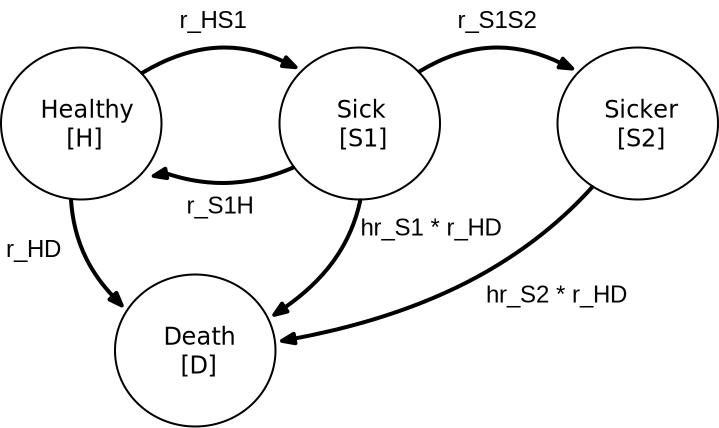
\includegraphics{index_files/mediabag/images/state-transition-diagram-1.pdf}

}

\caption{\label{fig-model1}State transition diagram for progressive
disease model}

\end{figure}%

\textsubscript{Source:
\href{https://graveja0.github.io/dalys/index.qmd.html}{Article
Notebook}}

\textsubscript{Source:
\href{https://graveja0.github.io/dalys/index.qmd.html}{Article
Notebook}}

\subsection{Transition Matrices}\label{transition-matrices}

With the model parameterized, our next step is to define the matrices
that govern health state transitions. The state transition diagram
represented in Figure~\ref{fig-model1} is not well-suited to calculate
DALY outcomes, however. A primary reason is that the death transitions
reflect transitions due to all causes of death. To calculate YLLs, we
need to separately track the timing and number of deaths \emph{due to
disease}.

To accommodate this need and to accurately model DALY outcomes, several
options are available. We categorize each approach based on the level of
experience and skill needed to execute it (beginner, intermediate,
advanced):

\begin{enumerate}
\def\labelenumi{\arabic{enumi}.}
\item
  \textbf{Separate Death State (Beginner)}: Re-define the health states
  to include a separate cause-specific death state as depicted in
  Figure~\ref{fig-modelDS}.\footnote{In this example, disease-specific
    death rates are goverened by a hazard ratio applied to the
    background mortality rate. Because we are operating on the rate
    scale, we can separate out disease-related deaths from other-cause
    mortality by simply taking a difference in the rates. Other
    applications for prevalent conditions with high death rates,
    however, may require us to construct a cause-deleted life table to
    obtain background mortality rates that net out deaths from the
    modeled disease.} We then draw on the resulting Markov trace and use
  changes in the number of cause-specific deaths in each cycle to
  calculate YLLs.
\item
  \textbf{Non-Markovian Trackers (Intermediate)}: Include a
  non-Markovian transition state for cause-specific deaths in the
  transition matrix. This approach will maintain the Markovian
  components captured in Figure~\ref{fig-model1}, but will allow us to
  add a column to the Markov trace that separately tracks the number of
  new deaths from the disease in each cycle. We can then apply
  transition state payoffs (based on remaining life expectancy at each
  age/cycle) to calculate YLL outcomes.
\item
  \textbf{Markov Chain with Rewards (Advanced)} Define a block matrix
  Markov chain with rewards for occupancy (YLDs) and disease-relatd
  death transitions (YLLs) by adapting the methods in Caswell \& van
  Daalen (2021). This approach draws on matrix calculus and solves for
  expected outcomes as well as higher order moments such as variance and
  skewness.
\end{enumerate}

Each of these approaches facilitate the design and execution of a
decision-analytic model that correctly calculates YLD, YLL, and DALY
outcomes---as well as other common outcomes such as QALYs and costs. In
practice, Approaches (1) and (2) will produce identical results.
Approach (3) draws on slightly different cycle correction techniques,
but will yield results quite similar to (1) and (2). Other shortcut
approaches previously used in the literature, such as modeling a
QALY-like DALY and/or accumulating time in the absorbing death state,
will not in general yield similar results; we discuss reasons for this
in Section TK below.

\subsubsection{Approach 1 (Beginner): Cause-Specific Death
State}\label{approach-1-beginner-cause-specific-death-state}

Under this approach, we separate out deaths from disease vs.~other
causes by defining a separate health state for cause-specific mortality;
an updated state transition diagram is shown in
Figure~\ref{fig-modelDS}.

\begin{figure}

\centering{

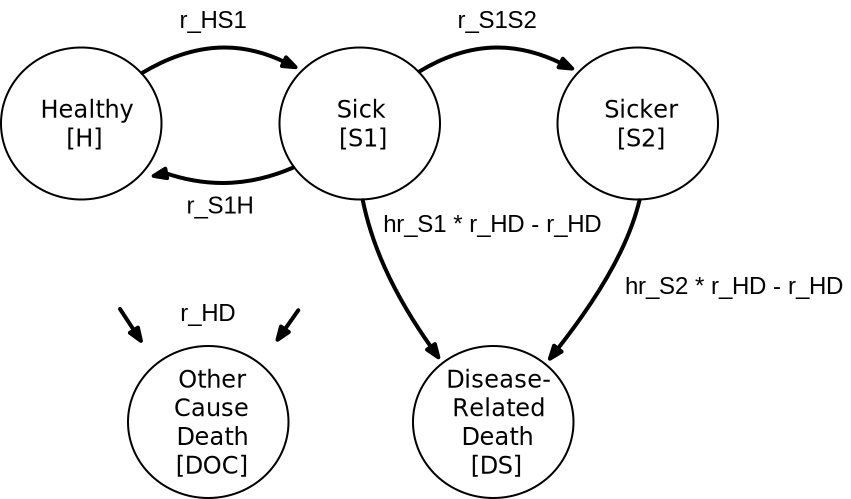
\includegraphics{index_files/mediabag/images/state-transition-diagram-2.pdf}

}

\caption{\label{fig-modelDS}State transition diagram for progressive
disease model with separate cause-specific death state}

\end{figure}%

Transitions among health states are defined in terms of continuous rates
(``intensities'') and are captured within an intensity matrix
\(\mathbf{Q}\),

\begin{figure}[H]

{\centering 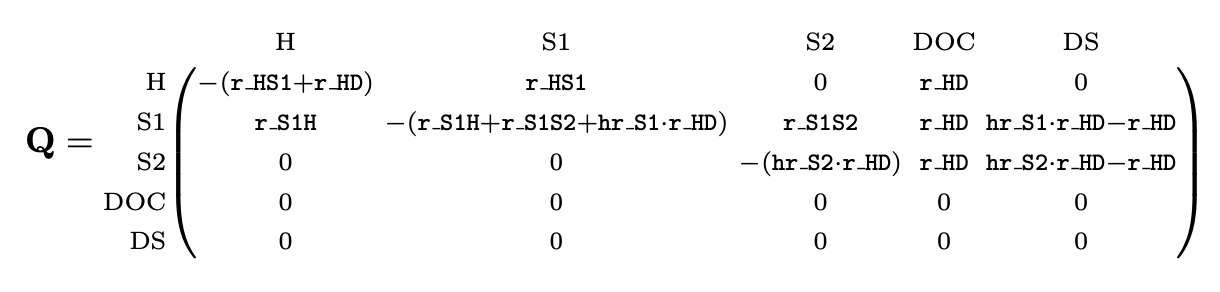
\includegraphics{images/Q_model2.png}

}

\caption{Transition Intensity Matrix for Approach 1}

\end{figure}%

Cell values in row \(i\), column \(j\) of \(\mathbf{Q}\) capture the
(continuous time) transition rate from health state \(i\) to health
state \(j\). \(\mathbf{Q}\) has diagonal elements defined as the
negative sum of the off-diagonal row values (i.e., the row sums of
\(\mathbf{Q}\) are zero). This ensures that the Markov model is
``closed''---that is, the total cohort size neither grows nor shrinks
over time.

We next embed the continuous transition intensity matrix into a discrete
time transition probability matrix by taking the matrix exponential of
\(\mathbf{Q}\) for a defined time step (i.e., ``cycle length'')
\(\Delta t\):\footnote{In Markov theory, \(\mathbf{P}\) is called the
  ``discrete skeleton'' of the continuous model (Iosifescu, 1980). The
  conversion formula used to calculate \(\widetilde{\mathbf{P}}\) is the
  matrix analogue to the standard rate-to-probability formula commonly
  taught in health economics textbooks, i.e., \(p = 1 - e^{r\Delta t}\),
  where \(r\) is the rate and \(\Delta t\) is the time step (i.e.,
  ``cycle length'').}

\begin{equation}\phantomsection\label{eq-embed}{
\mathbf{P} = e^{\mathbf{Q}\Delta t}
}\end{equation}

This results in a transition probability matrix with the following
probabilities defined:

\begin{figure}[H]

{\centering 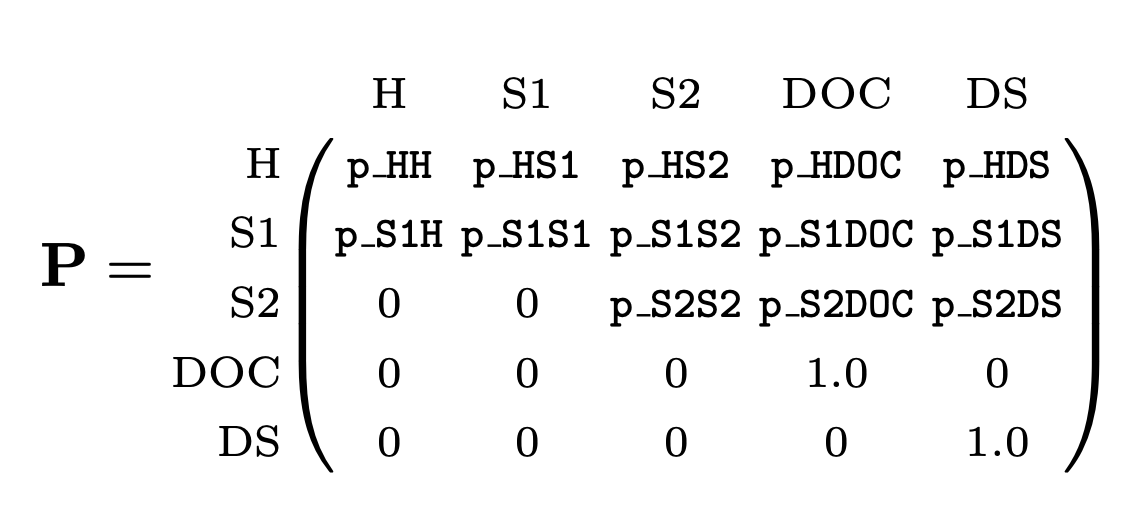
\includegraphics[width=0.6\textwidth,height=\textheight]{images/P_model2.png}

}

\caption{Transition Probability Matrix for Approach 1}

\end{figure}%

Embedding the transition probability matrix using the matrix exponential
ensures that the resulting transition probabilities capture the
underlying continuous time disease process. In particular,
\(\mathbf{P}\) will capture the probability of compound (``jumpover'')
transitions within a single cycle.

For example, in the continuous time rate matrix \(\mathbf{Q}\) above,
there is a zero-valued rate defined for progressions from Healthy (H) to
Disease-related death (DS), since individuals must first become ill
before they can die from disease-related causes. However, after
embedding, the matrix \(\mathbf{P}\) has a non-zero cycle transition
probability from Healthy (H) to Disease-related death (DS) (i.e.,
\(\texttt{p\_HDS}\)). This value captures the probability of a compound
or ``jumpover'' transition from Healthy and through the Sick and/or
Sicker state to death from disease-related causes within the same
discrete time cycle; see Graves et al. (2021) for further discussion,
and Iosifescu (1980) for additional theory.\footnote{Because we embed
  the transition probability matrix using matrix exponentiation, rather
  than through pairwise application of rate-to-probability formulas to
  each transition type, our results will differ from those in
  Alarid-Escudero et al. (2023)---even though we use identical input
  parameters. Application of standard rate-to-probability formulas in
  health states with competing risks (i.e., the possibility of
  transitioning to more than one other health state in a given cycle)
  will ignore the possibility of compound transitions within a single
  cycle. Though not (yet) widely used in health economics, embedding the
  transition probability matrix using the matrix exponential is the
  technically correct way to construct a transition probability matrix
  from underlying transition rates.}

\subsubsection{Approach 2 (Intermediate): Non-Markovian Tracking
States}\label{approach-2-intermediate-non-markovian-tracking-states}

This section will outline an approach similar to Approach 1, but that
draws on a non-Markovian ``transition'' state that tracks the number of
disease-related deaths in each cycle; these counts will be used later to
match the age of the cohort at each cycle with a reference life table to
calculate YLL outcomes.

Under this approach, we maintain the overall structure as depicted in
the original model (Figure~\ref{fig-model1}), but augment the transition
probability matrix with non-Markovian components to facilitate
accounting of disease-related deaths.\footnote{Tracking states also
  allow for accurate bookeeping for other outcomes such as costs. For
  example, if developing the disease incurs a one-time diagnosis or
  treatment cost, the compound transitions implied by the embedded
  transition probability matrix indicate that some individuals will
  transiently enter (and then exit) the Sick state in a single cycle.
  When calculating costs, practitioners may want to include a tracking
  state for the Sick state to be sure to capture these one-time costs,
  which would be masked if cost payoffs are simply multiplied by state
  occupancy at the end of each cycle (e.g., costs for individuals with a
  sojourn through the Sick state in a single cycle would not be
  accounted for).} Approach 2 offers a more generalized method that
allows practitioners to accurately account for costs and/or health
payoffs (such as YLLs) that are defined by \emph{transitions} among
health states, rather than occupancy in a health state.

Figure~\ref{fig-transition} shows a state transition diagram with the
tracking state added. The tracking state (shown as red nodes) simply
records transitions as cohort members move from either diseased state to
the absorbing death state due to causes related to the disease.

\begin{figure}

\centering{

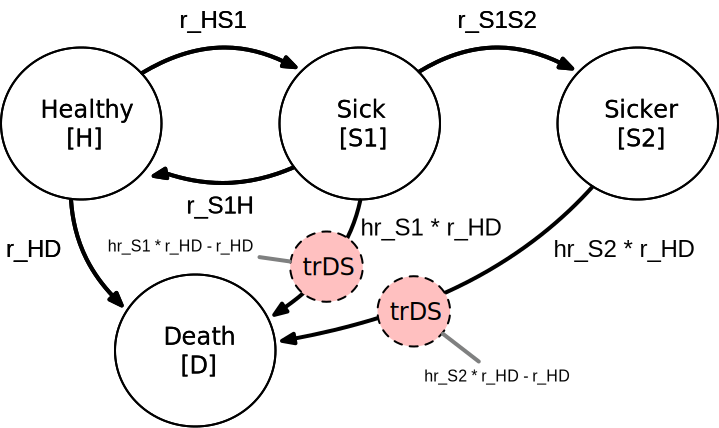
\includegraphics{index_files/mediabag/images/state-transition-diagram-3.pdf}

}

\caption{\label{fig-transition}State Transition Diagram with Transition
State (Red)}

\end{figure}%

In general, tracking states can either count the total number of
transitions that have occurred up to a given cycle (i.e., an
``accumulator'' state), or can track the total number of new transitions
that occur within a single cycle (i.e., a ``transition''
state).\footnote{More generally, accumulator and transition states can
  be defined for any number of transition types, as they are useful for
  capturing one-time costs in the model, or for for calculating other
  decision-relevant outcomes such as the total number of people who
  developed the disease or died from the disease as secondary outcomes.}
To calculate YLL outcomes we will add a transition state that records
the total number of new disease-related deaths in each cycle.

To implement Approach 2, we add a transition state row and column to the
transition intensity matrix. This transition state, called
\(\texttt{trDS}\), is included in the augmented intensity matrix
\(\mathbf{Q}\) below:

\begin{figure}[H]

{\centering 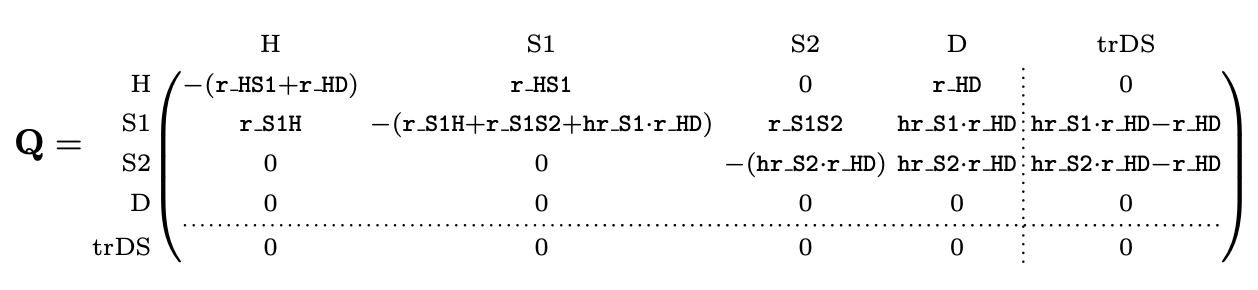
\includegraphics{images/Q_model1.png}

}

\caption{Transition intensity matrix with transition state added}

\end{figure}%

Two aspects of \(\mathbf{Q}\) are worth highlighting. First,
\(\mathbf{Q}\) is divided into a Markovian submatrix and the
non-Markovian tracking row and column. This division is made apparent
using dotted vertical and horizontal lines. Critically, the Markovian
submatrix remains closed---that is, the diagonal elements remain
unchanged so that the row sums of the submatrix remain zero, even after
the addition of the tracking column along the ``edges'' of
\(\mathbf{Q}\). This ensures that the Markovian submatrix can be used to
calculate state occupancy for a closed cohort that neither gains nor
loses cohort members over the modeled time horizon.

Second, two transition intensities---from the S1 (Sick) and S2 (Sicker)
states to Death---appear in the tracking column. This ensures that
\(\texttt{trDeadDisease}\) will track all relevant transitions to death
due to the disease. Because we are operating on the rate scale, we can
net out non-disease related deaths as captured by the background
mortality rate among healthy individuals (i.e., \(\texttt{r\_HD}\)).

As above, we obtain the transition probability matrix by embedding
\(\mathbf{Q}\) into the discrete time step (Equation~\ref{eq-embed}).
However, the resulting transition probability matrix treats
\(\texttt{trDS}\) as an absorbing state (i.e., individuals are retained
in the \(\texttt{trDS}\) with probability one). Using the terminology
introduced above, this absorbing state could serve as an
\textbf{accumulator} state that (in the constructed Markov trace)
records the total number of people who have died from the disease up to
any given cycle. This may be a decision-relevant health outcome to
consider on its own; indeed, so long as the Markovian submatrix remains
closed, there is no limit to the number of accumulator and/or transition
states one might add along the ``edges'' of a model.\footnote{To build
  on the example of compound ``jumpover'' transitions above, suppose an
  individual starts off healthy in a cycle, then rapidly transitions
  through the Sick and Sicker state and dies due to disease-related
  causes within the same cycle. If there is some treatment cost
  associated with being in the Sicker state, a traditional approach that
  applies cost payoffs to state occupancy at the (beginning) end of the
  cycle would miss treatment costs for this individual because they
  \emph{transition} through the Sicker state, but never occupy it at the
  beginning or end of a cycle. Adding a non-Markovian transition state
  to the model facilitates more accurate bookkeeping because the
  transition state would pick up on this transition through the Sicker
  state.}

To change \(\texttt{trDS}\) to a \textbf{transition} state, we simply
replace the absorbing probability of one in the cell
\([\texttt{trDS},\texttt{trDS}]\) with a zero. This cell-level change is
highlighted in grey in the bottom right cell of \(\mathbf{P}\) below:

\begin{figure}[H]

{\centering 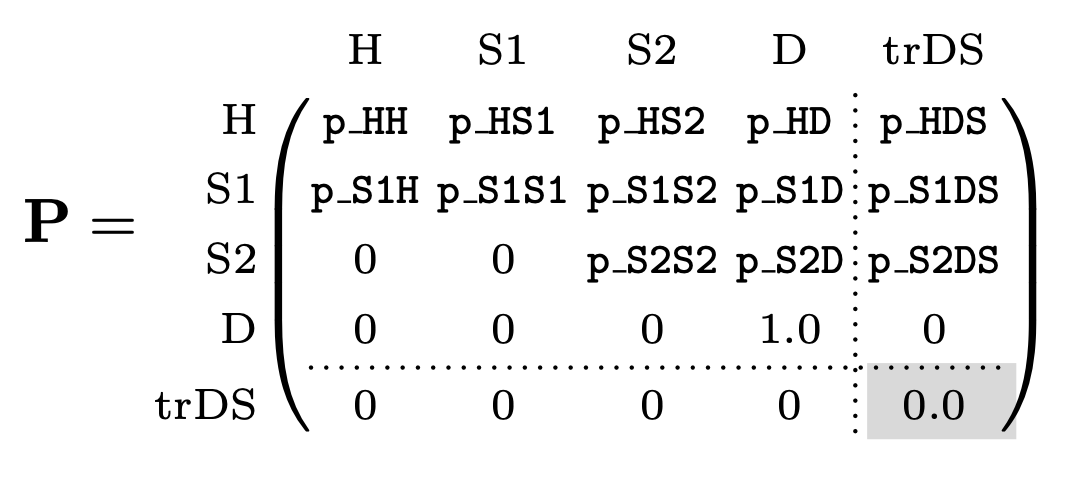
\includegraphics[width=0.6\textwidth,height=\textheight]{images/P_model1.png}

}

\caption{Transition Probability Matrix for Approach 2}

\end{figure}%

\textsubscript{Source:
\href{https://graveja0.github.io/dalys/index.qmd.html}{Article
Notebook}}

\subsubsection{Approach 3 (Advanced): Markov Chain With
Rewards}\label{approach-3-advanced-markov-chain-with-rewards}

Define

\[
\begin{aligned}
\tau &= \text{Number of transient (non-absorbing) states}\\
\alpha &= \text{Number of absorbing states}\\
\omega &= \text{Number of cycles} \\
s &= \text{Total number of states; }s=\tau\omega+\alpha \\
\mathbf{U}_{x} &= \text{Transition matrix for age }x, \text{for }x=1,\dots,\omega\\
\mathbf{D}_{j} &=\text{Age advancement matrix for stage }j, \text{for }j=1,\dots,\tau \\
\mathbf{M}_{i} &= \text{Mortality matrix for age class }x, \text{for } x = 1,\dots\omega \\
\mathbf{K} &= \text{vec-permutation matrix; parameters }\tau,\omega
\end{aligned}
\] In the above notation, the matrix \(\mathbf{U}_x\) captures
transition probabilities among transient (i.e., non-absorbing) health
states, while \(\mathbf{M}_x\) captures transitions from transient
health states to the absorbing death states (non-disease mortality and
disease-related mortality). Indexing by age class \(x\) indicates that
separate matrices are defined for each age in the Markov model.

To construct \(\mathbf{U}_x\) and \(\mathbf{M}_x\) we define transition
rate (``intensity'') matrices as in Approaches 1 and 2 above.\footnote{The
  only difference with the two approaches above is that the rows in
  these rate matrices correspond to the final state, while the columns
  correspond to the starting state; this is the opposite of the rate
  matrices defined above, where the rows corresponded to the starting
  health state and the columns to the ending health state in a given
  cycle.} The overall intensity matrix \(\mathbf{Q_x}\) is given by

\[
\mathbf{Q}_x=\left(\begin{array}{c|c}
\mathbf{V}_x & \mathbf{0} \\
\hline \mathbf{S}_x  & \mathbf{0}
\end{array}\right)
\] where \(\mathbf{V}_x\) is the rate matrix for the transitory (i.e.,
non-absorbing) states and \(\mathbf{S}_x\) is the rate matrix for the
absorbing states. The diagonal elements of \(\mathbf{Q}_x\) are the
negative sum of the non-diagonal column elements, thus making the column
sums of \(\mathbf{Q}_x\) zero.

For the defined time step \(\Delta_t\), the discrete time transition
probability matrix \(\mathbf{P}_x\) is obtained by taking the matrix
exponential of the intensity matrix (\(\mathbf{Q}_x\)) multipled by the
time step (\(\Delta_t\)):

\[
\mathbf{P}_x =e^{\mathbf{Q}_x  \Delta t}
\]

We can then obtain \(\mathbf{U}_x\) and \(\mathbf{M}_x\) based on:

\[
\mathbf{P}_x =\left(\begin{array}{c|c}
\mathbf{U}_x  & \mathbf{0} \\
\hline \mathbf{M}_x  & \mathbf{0}
\end{array}\right)
\]

In addition, the matrix \(\mathbf{D}_j\) defines age advancement in the
Markov chain. Using the example from Caswell \& van Daalen (2021), if
\(\omega=3\) then

\[
\mathbf{D}_j=\left(\begin{array}{ccc}
0 & 0 & 0 \\
1 & 0 & 0 \\
0 & 1 & {[1]}
\end{array}\right) \quad j=1, \ldots, \tau
\]

In our implementation, we include the (optional) 1 value in the lower
right corner; this assumes that after the last specified age, the cohort
continues to experience transitions among health states according to the
transition probabilities defined for the last age class. If this value
is 0, the model will assume that everyone dies after the last cycle.

We next combine the transition matrices (for all age classes) together
into a series of block-structured matrices as follows:

\[
\mathbb{U}=\left(\begin{array}{c|c|c}
\mathbf{U}_1 & \cdots & \mathbf{0} \\
\hline & \ddots & \\
\hline \mathbf{0} & \cdots & \mathbf{U}_\omega
\end{array}\right)
\]

\[
\mathbb{D}=\left(\begin{array}{c|c|c}
\mathbf{D}_1 & \cdots & \mathbf{0} \\
\hline & \ddots & \\
\hline \mathbf{0} & \cdots & \mathbf{D}_\tau
\end{array}\right)
\]

\[
\tilde{\mathbf{U}}=\mathbf{K}^{\top} \mathbb{D} \mathbf{K} \mathbb{U} \quad \tau \omega \times \tau \omega
\]

where \(\mathbf{K}\) is a permutation matrix known as the
vec-permutation matrix.\footnote{A function to construct a
  vec-permultation matrix is provided within the code snippet below.}
See Henderson \& Searle (1981) and Appendix B in Caswell \& van Daalen
(2021) for further information.

We also define

\[
\tilde{\mathbf{M}}=\left(\begin{array}{lll}
\mathbf{M}_1 & \cdots & \mathbf{M}_\omega
\end{array}\right) \quad \alpha \times \tau \omega
\]

and

\[
\tilde{\mathbf{P}}=\left(\begin{array}{c|c}
\tilde{\mathbf{U}} & \mathbf{0}_{\tau \omega \times \alpha} \\
\hline \tilde{\mathbf{M}} & \mathbf{I}_{\alpha \times \alpha}
\end{array}\right) \quad(\tau \omega+\alpha) \times(\tau \omega+\alpha)
\] where \(\mathbf{I}\) is the identity matrix and \(\mathbf{0}\) is a
matrix of zeros.

We now (nearly) have the components needed to calculate outcomes. A key
difference in the Healthy Longevity approach, relative to the approaches
above, is that we do not calculate outcomes separately in each cycle,
and then sum them. Rather, the method utilizes matrix calculus to solve
for \emph{expected outcomes} and other moments in the outcome
distribution (e.g., variance, skewness, etc.).\footnote{Again, for our
  purposes here we will focus on expected outcomes---though note that
  formulas for higher-order moments are provided in Caswell \& van
  Daalen (2021) and Caswell \& Zarulli (2018).}

\textsubscript{Source:
\href{https://graveja0.github.io/dalys/index.qmd.html}{Article
Notebook}}

\subsection{Outcomes}\label{outcomes}

With \(\mathbf{P}\) defined under either Approach 1 or Approach 2, we
now have the necessary ingredients to construct a Markov trace. Define
\(\mathbf{s}_0\) as the initial state occupancy vector at time \(t=0\).
The vector \(\mathbf{s}_0\) has size \(k\), where \(k\) is the total
number of states captured in the \(k \times k\) matrix \(\mathbf{P}\)
(including transition states, if using Approach 2). This vector
summarizes the number or fraction of the population in each health state
at baseline. Often, this vector will be set such that the entire cohort
starts off healthy---though this need not always be the case.

For a time-homogenous model such as considered here, health state
occupancy at cycle \(t\) is is calculated as:

\begin{equation}\phantomsection\label{eq-trace}{
\mathbf{s}'_t=\mathbf{s}'_0 \mathbf{P}^t
}\end{equation}

For a time-inhomongenous model in which transition probabilities change
over time (e.g., death rates increase due to aging), we must construct
separate transition probability matrices for each cycle (i.e.,
\(\mathbf{P}(t)\)). State occupancy at cycle \(t\) is calculated by
sequentially applying the transition matrices corresponding to each time
step leading up to cycle \(t\), i.e.,

\begin{equation}\phantomsection\label{eq-trace-inhomo}{
\mathbf{s}'_t=\mathbf{s}'_0 \mathbf{P}(1)\mathbf{P}(2)\dots\mathbf{P}(t)
}\end{equation}

\subsubsection{Years of Life Lived with Disability
(YLD)}\label{years-of-life-lived-with-disability-yld}

To calculate YLDs, we define a disability weight payoff vector
\(\mathbf{d}_{YLD}\),

\begin{figure}[H]

{\centering 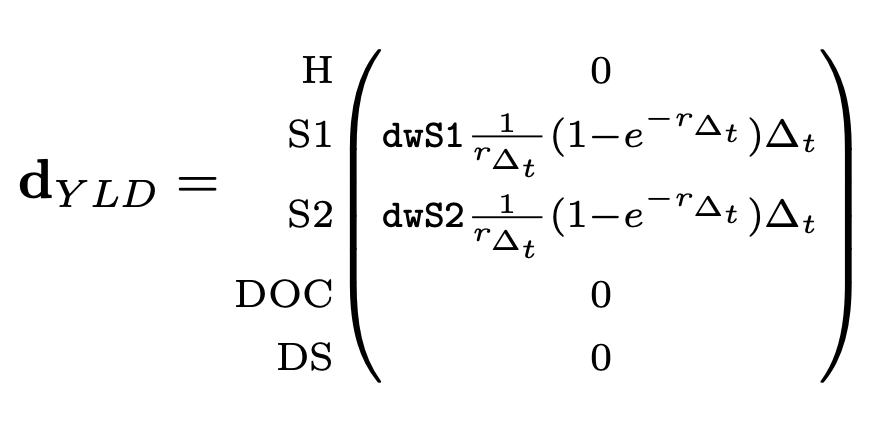
\includegraphics[width=0.6\textwidth,height=\textheight]{images/d_yld.png}

}

\caption{YLD Payoff Vector}

\end{figure}%

where \(\texttt{dwS1}\) and \(\texttt{dwS2}\) are the disability weights
for the Sick and Sicker states, respectively. In addition,
\(r_{\Delta_t}\) is the cycle discount rate, which is calculated as,

\begin{equation}\phantomsection\label{eq-cycledisc}{
r_{\Delta_t} = r \Delta_t
}\end{equation} where \(r\) is the annual discount rate and \(\Delta_t\)
is the time step.

In the YLD payoff vector, the term
\(\frac{1}{r_{\Delta_t}}(1-e^{-r_{\Delta_t}})\) is included as a
continuous-time discounting adjustment factor for the defined cycle
length \(\Delta_t\). This term is included to discount time
\emph{within} each cycle in order to maintain the continuous-time
discounting approach used in the original GBD equations.\footnote{For
  example, if \(r=0.03\) and \(\Delta_t=1\) (i.e., annual cycle length),
  this adjustment factor will be
  \(0.985 = \frac{1}{r_{\Delta_t}}(1-e^{-r_{\Delta_t}})\). If
  \(\Delta_t=1/12\) (monthly cycle) the cycle discounting adjustment
  factor is 0.99875.}

To fully discount outcomes, we still must discount all future outcome
values back to baseline (\(t=0\)). For a time-homogeneous model,
discounted years of life lost to disability (YLD) at cycle \(t\) is
given by

\begin{equation}\phantomsection\label{eq-yldt}{
YLD(t)=\mathbf{s}'_0 \mathbf{P}^t \mathbf{d}_{YLD}  \times{e^{-r_{\Delta_t} t}}
}\end{equation}

For a time-inhomogenous model, YLDs are calculated as
\begin{equation}\phantomsection\label{eq-yldt-inhomo}{
YLD(t)=\mathbf{s}'_0 \mathbf{P}(1)\mathbf{P}(2)\dots\mathbf{P}(t)  \mathbf{d}_{YLD}  \times{e^{-r_{\Delta_t} t}}
}\end{equation}

\subsubsection{Years of Life Lost to Disease
(YLLs)}\label{years-of-life-lost-to-disease-ylls}

As noted in Section~\ref{sec-background} and in Equation~\ref{eq-yll},
YLLs are based on the present value of remaining life expectancy among
deaths that occur in each cycle \(t\). Define \(a(t)\) as the age of the
cohort at cycle \(t\), i.e., \(a(t) = t \cdot \Delta t + a0\), where
\(a_0\) is the age of the cohort at \(t=0\). Define \(e(t)=e(a(t))\) as
the present value of remaining life expectancy at cycle \(t\). Following
the GBD continuous time discounting approach, \(e(a(t))\) is given by

\begin{equation}\phantomsection\label{eq-pvEx}{
e(a(t)) = \frac{1}{r}\big (1 - e^{-rEx(a(t))} \big )
}\end{equation}

where \(Ex(a)\) is the remaining life expectancy at age \(a\). \(Ex(a)\)
is drawn from either an exogenous (reference) or an endogenous life
table, depending on the objectives of the modeling exercise (Anand \&
Reddy, 2019).

We next define a remaining life expectancy payoff vector at cycle \(t\):

\begin{figure}[H]

{\centering 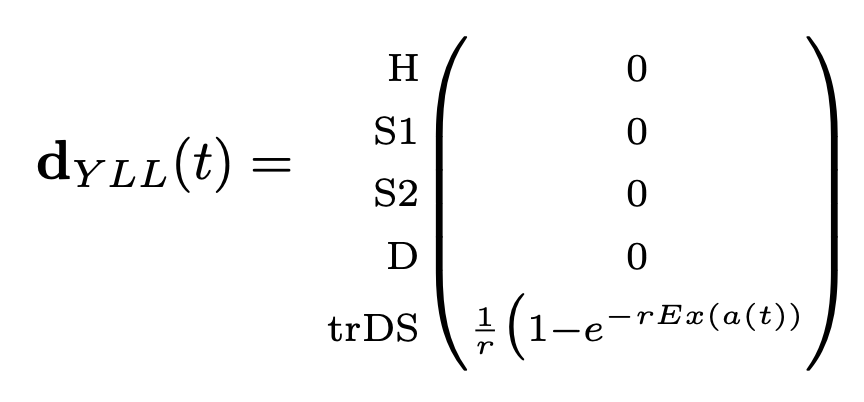
\includegraphics[width=0.6\textwidth,height=\textheight]{images/d_yll.png}

}

\caption{YLL Payoff Vector}

\end{figure}%

This payoff vector reflects discounting, but only in terms of the
present value of remaining life expectancy \emph{at time} \(t\).

\begin{equation}\phantomsection\label{eq-yllt}{
YLL(t)=\mathbf{s}'_t \mathbf{e}(t)  \times{e^{-r\Delta_t t}} =\mathbf{s}'_0 \mathbf{P}^t \mathbf{e}(t)  \times{e^{-r\Delta_t t}}
}\end{equation}

Total discounted YLLs at time \(t=0\) is given by:

\begin{equation}\phantomsection\label{eq-yllcum}{
YLL=\sum_{t=0}^{N-1} YLL(t) =\sum_{t=0}^{N-1}\left(\mathbf{s}'_0 \mathbf{P}^t \mathbf{e}(t)  \times{e^{-r\Delta_t t}} \right) 
}\end{equation}

\textsubscript{Source:
\href{https://graveja0.github.io/dalys/index.qmd.html}{Article
Notebook}}

\textsubscript{Source:
\href{https://graveja0.github.io/dalys/index.qmd.html}{Article
Notebook}}

To calculate outcomes, we must next define ``reward'' matrices
\(\mathbf{R}_m\), where \(m\) indexes the moment of interest (e.g.,
expected value, variance, etc.). The structure and values of
\(\mathbf{R}_m\) will differ, however, depending on the outcome.

To facilitate how we define rewards (i.e., payoffs), we briefly classify
each of our outcomes (LE, YLL, YLD, DALYs, QALYs) into broad classes
corresponding to whether the payoff or ``reward'' applies to occupancy,
or to transitions, within or to a given health state:

\begin{longtable}[]{@{}
  >{\raggedright\arraybackslash}p{(\columnwidth - 2\tabcolsep) * \real{0.3750}}
  >{\raggedright\arraybackslash}p{(\columnwidth - 2\tabcolsep) * \real{0.6250}}@{}}
\caption{Classification of Health Outcomes}\tabularnewline
\toprule\noalign{}
\begin{minipage}[b]{\linewidth}\raggedright
Outcome
\end{minipage} & \begin{minipage}[b]{\linewidth}\raggedright
Reward Class
\end{minipage} \\
\midrule\noalign{}
\endfirsthead
\toprule\noalign{}
\begin{minipage}[b]{\linewidth}\raggedright
Outcome
\end{minipage} & \begin{minipage}[b]{\linewidth}\raggedright
Reward Class
\end{minipage} \\
\midrule\noalign{}
\endhead
\bottomrule\noalign{}
\endlastfoot
Life Expectancy & Occupancy (1.0 for each alive health state) \\
Years of life lived with disability (YLD) & Occupancy (disability weight
applied to time in CVD state) \\
Yearls of life lost to disease (YLL) & Transition (remaining life
expectancy applied to CVD death transitions) \\
Disability-Adjusted Life Years (DALYs) & Occupancy (YLD) + Transition
(YLL) \\
Quality-Adjusted Life Years & Occupancy (utility weights applied to
living health states) \\
\end{longtable}

\subsubsection{Occupancy-Based Outcomes}\label{occupancy-based-outcomes}

To calculate occupancy-based outcomes, we start with a reward matrix
\(\mathbf{H}\), which has dimensions \(\tau \times \omega\) and is
structured as shown in Figure~\ref{fig-H-le}:

\begin{figure}

\centering{

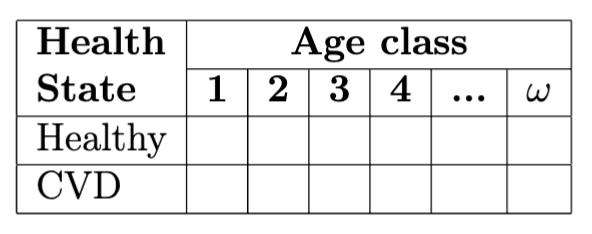
\includegraphics[width=0.5\textwidth,height=\textheight]{images/H-LE.png}

}

\caption{\label{fig-H-le}Reward matrix \(\mathbf{H}\)}

\end{figure}%

Cell values within this matrix can be set to one if we want to
``reward'' that health state-age combination in our outcome measure, and
zero otherwise.\footnote{This structure allows us, for example, to
  estimate outcomes for certain age ranges or other decision-relevant
  combinations of health state and age.}

For occupancy-based outcomes, we define \(\mathbf{H}\) such that each
cell receives a value of one.

\begin{figure}

\centering{

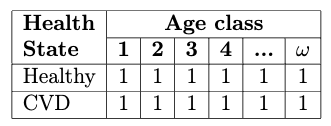
\includegraphics[width=0.5\textwidth,height=\textheight]{images/H-LE2.png}

}

\caption{\label{fig-H}Reward matrix \(\mathbf{H}\)}

\end{figure}%

We use this matrix to define the reward vector
\(\mathbf{h}\):\footnote{The \(\text{vec}\) operator stacks the columns
  of an \(m \times n\) matrix into a \(mn \times 1\) vector.}

\[
\mathbf{h} = \text{vec } \mathbf{H}
\] We also define \(\neg \mathbf{h}\) as the complement of
\(\mathbf{h}\), (i.e., values of 1.0 become 0, and vice versa).

Occupancy-based outcomes with partial rewards (e.g., YLDs, QALYs)
require an additional matrix \(\mathbf{V}\), which has the same
structure as \(\mathbf{H}\):

If \(\mathbf{S}\) is the set of states that receive a reward (e.g., the
CVD state for both QALYs and YLDs), then a cycle spent in state \(i\) at
age \(j\) is defined by

\[
\mathbf{V}(i, j)= \begin{cases}E\left[v(i, j)\right] & \text { if }(i, j) \in \mathcal{S} \\ 0 & \text { otherwise }\end{cases}
\] For YLD outcomes, \(\mathbf{V}\) is defined as shown in
Figure~\ref{fig-V-yld}, while for QALY outcomes \(\mathbf{V}\) is
defined as shown in Figure~\ref{fig-V-qaly} .

\begin{figure}

\centering{

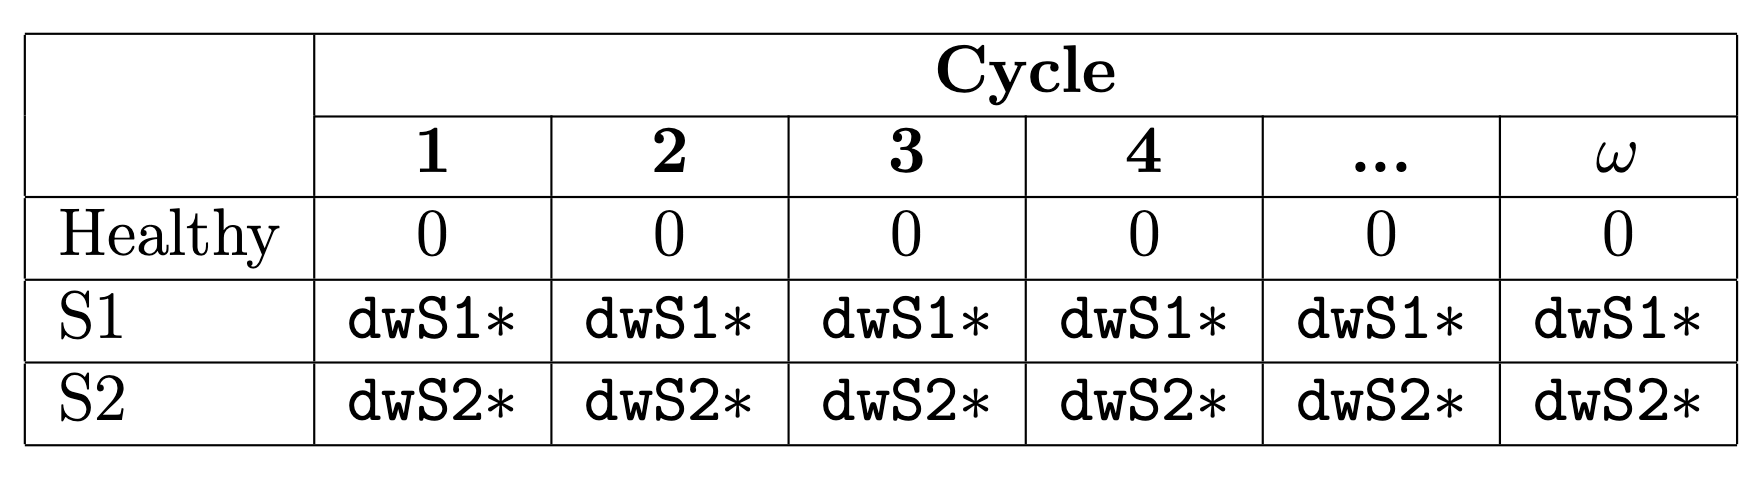
\includegraphics[width=0.7\textwidth,height=\textheight]{images/H-YLD.png}

}

\caption{\label{fig-V-yld}Reward matrix for YLD Outcome}

\end{figure}%

\begin{figure}

\centering{

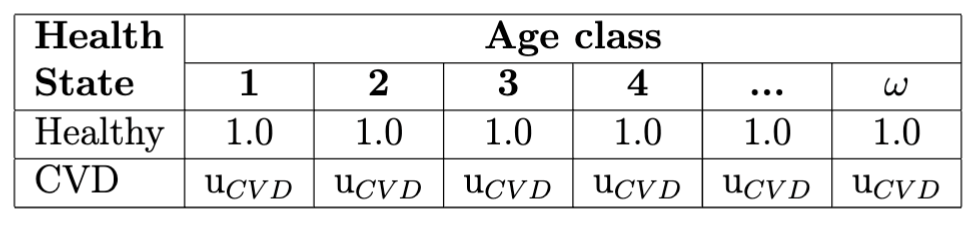
\includegraphics[width=0.6\textwidth,height=\textheight]{images/H-QALY.png}

}

\caption{\label{fig-V-qaly}Reward matrix \mathbf{V} for QALY Outcome}

\end{figure}%

We simliarly define an occupancy indicator vector \(\mathbf{v}\) just as
we did \(\mathbf{h}\):

\[
\mathbf{v}_{m}=\operatorname{vec} \mathbf{V}_{m}
\]

\subsubsection{Rewards for Partial
Occupancy}\label{rewards-for-partial-occupancy}

Like many health economic applications, the Healthy Longevity approach
makes assumptions on partial occupancy in a health state.\footnote{For
  example, half-cycle corrections are often used---though there are
  other methdos (e.g., Simpson's rule) that are also drawn upon.}
Specifically, the approach assumes that partial occupancy in a health
state receives half the reward---essentially, we draw on an assumption
that mid-cycle transitions occur at the half-way point.\footnote{This is
  similar to the standard ``half-cycle'' correction, however under this
  approach, a half-cycle correction occurs in each cycle, not in the
  first and last cycles. As we will see below, for rewards that are
  uniform across transient health states (e.g., calculating life
  expectancy involves a ``payoff'' of 1.0 for every living health state)
  this will yield identical answers as a Markov trace-based approach
  that adopts a half-cycle correction.}

We combine this partial ocupancy assumption, along with the vectorized
reward matrices \(\mathbf{h}\) and \(\mathbf{v}\) to obtain the
following:

\[
\begin{aligned}
\tilde{\mathbf{B}}_{1} & =\mathbf{h} \mathbf{v}_{1}^{\top}+\frac{1}{2}(\neg \mathbf{h})\left(\mathbf{v}_{1}^{\top}\right)+\frac{1}{2}\left(\mathbf{v}_{1}\right)\left(\neg \mathbf{h}^{\top}\right) \\
\end{aligned}
\] and

\[
\tilde{\mathbf{C}}_{1}=\frac{1}{2} \mathbf{1}_{\alpha} \mathbf{v_1}^{\top}
\]

We combine \(\tilde{\mathbf{B}}_{1}\) and \(\tilde{\mathbf{C}}_{1}\) to
obtain:

\[
\tilde{\mathbf{R}}_{1}=\left(\begin{array}{c|c}
\tilde{\mathbf{B}}_{1} & \mathbf{0} \\
\hline \tilde{\mathbf{C}}_{1} & \mathbf{0}
\end{array}\right) 
\] which has same block structure as the transition probability matrix
\(\tilde{\mathbf{P}}\).

Expected outcomes are based on

\[
\begin{aligned}
& \tilde{\boldsymbol{\rho}}_{1}=\tilde{\mathbf{N}}^{\top} \mathbf{Z}\left(\tilde{\mathbf{P}} \circ \tilde{\mathbf{R}}_{1}\right)^{\top} \mathbf{1}_{s} 
\end{aligned}
\] where \(\tilde{\mathbf{N}}\) is the fundamental matrix

\[
\tilde{\mathbf{N}}=(\mathbf{I}-\tilde{\mathbf{U}})^{-1}
\] and \(\mathbf{Z}\) is

\[
\mathbf{Z}=\left(\mathbf{I}_{\tau \omega} \mid \mathbf{0}_{\tau \omega \times \alpha}\right)
\]

\subsubsection{Transition-Based
Outcomes}\label{transition-based-outcomes}

For transition-based outcomes such as YLLs, we define the first moment
of remaining life expectancy as the vector
\(\tilde{\boldsymbol{\eta}}^{\top}\). This vector has dimensions
\(\tau\omega \times 1\) and has the following basic structure:

\[
\tilde{\mathbf{\eta}}=\left(\begin{array}{c}
\eta_{11} \\
\vdots \\
\eta_{\tau 1} \\
\hline \vdots \\
\hline \eta_{1 \omega} \\
\vdots \\
\eta_{\tau \omega}
\end{array}\right)
\] where \(\eta_{i x}\) is remaining life expectancy for an individual
in health state \(i\) at a given age \(x\). In this structure, remaining
life expectancy for each health state is grouped within age classes.

Our choice for remaining life expectancy values \(\eta_{i x}\) for YLL
outcomes will depend on the context and research question at hand (Anand
\& Reddy, 2019). Historically, the GBD has utilized an \emph{exogenous},
external life table based on the maximum potential life span among
humans (Global Burden of Disease Collaborative Network, 2021). Anand \&
Reddy (2019) discuss alternative contexts in which remaining life
expectancy based on an \emph{endogenous} life table or life expectancy
model might be preferred.

The distinction between \emph{exogenous} and \emph{endogenous} rewards
for YLLs boils down to whether the remaining life expectancy value used
originates from \emph{outside} the population under study (i.e.,
mortality risks used to calculate remaining life expectancy at a given
age are independent of the mortality risks of the population being
assessed), or not.

For YLLs based on exogenous life tables, such as the reference life
table published by the GBD, we define
\(\tilde{\boldsymbol{\eta}}^{\top}\) based on the reference life table
value at each age. For YLLs based on an endogenous life table, we could
simply swap in external life table values from our country or region of
interest, \emph{or} use the model itself to estimate remaining life
expectancy for a given age and initial health state.

We next construct the reward matrices:

\[
\begin{aligned}
\tilde{\mathbf{B}}_{1} & =\left(\mathbf{0}_{\tau \omega \times \tau \omega}\right) \\
\tilde{\mathbf{C}}_{1} & =\left(\begin{array}{c}
\tilde{\boldsymbol{\eta}}_{1}^{\top} \\
\mathbf{0}_{1 \times \tau \omega}
\end{array}\right) .
\end{aligned}
\]

and

\[
\tilde{\mathbf{R}}_{1}=\left(\begin{array}{c|c}
\mathbf{0}_{\tau \omega \times \tau \omega} & \mathbf{0}_{\tau \omega \times 2} \\
\hline \tilde{\boldsymbol{\eta}}_{1}^{\top} & \mathbf{0}_{1 \times 2} \\
\mathbf{0}_{1 \times \tau \omega} & \mathbf{0}_{1 \times 2}
\end{array}\right)
\]

Echoing the approach to occupancy-based rewards above, expected outcomes
are based on

\[
\begin{aligned}
& \tilde{\boldsymbol{\rho}}_{1}=\tilde{\mathbf{N}}^{\top} \mathbf{Z}\left(\tilde{\mathbf{P}} \circ \tilde{\mathbf{R}}_{1}\right)^{\top} \mathbf{1}_{s} 
\end{aligned}
\] where \(\circ\) denotes element-wise multiplication,
\(\tilde{\mathbf{N}}\) is the fundamental matrix

\[
\tilde{\mathbf{N}}=(\mathbf{I}-\tilde{\mathbf{U}})^{-1}
\] and \(\mathbf{Z}\) is

\[
\mathbf{Z}=\left(\mathbf{I}_{\tau \omega} \mid \mathbf{0}_{\tau \omega \times \alpha}\right)
\]

\subsection{Total Expected Outcomes}\label{total-expected-outcomes}

For both occupancy- and transition-based outcomes, total (across all
ages) outcomes for each starting health state are calculated as

\[
\boldsymbol{\rho}_{m}^{\text {stage }}(\operatorname{age} x)=\left(\mathbf{e}_{x}^{\top} \otimes \mathbf{I}_{\tau}\right) \tilde{\boldsymbol{\rho}}_{m} \quad \tau \times 1
\] where \(\otimes\) is the Kronecker operator.

Alternatively, we may wish to calculate outcomes separately under
different starting ages, and for a specified starting health state
(e.g., healthy). This is given by

\[
\boldsymbol{\rho}_{m}^{\text {age }}(\text { stage } i)=\left(\mathbf{I}_{\omega} \otimes \mathbf{e}_{i}^{\top}\right) \tilde{\boldsymbol{\rho}}_{m} \quad \omega \times 1,
\]

\textsubscript{Source:
\href{https://graveja0.github.io/dalys/index.qmd.html}{Article
Notebook}}

\subsection{Results}\label{results}

Table~\ref{tbl-trace1} shows the Markov trace for the first five cycles
under Approach 1, while Table~\ref{tbl-trace2} shows the trace under
Approach 2. Table~\ref{tbl-trace1} also includes a new column
(\texttt{deaths\_disease}) that is calculated as the difference in state
occupancy in the \texttt{DS} column between cycles. This extra step will
be necessary later for calculating YLL outcomes. The trace shown under
Approach 2 (Table~\ref{tbl-trace2}), by comparison, automatically
calculates new deaths through the inclusion of the transition state
\texttt{trDS}; the values under \texttt{deaths\_disease} and
\texttt{trDS} are identical, again highlighting that either approach can
be used to calculate the number of disease-related deaths in each cycle.

\begin{table}

\caption{\label{tbl-trace1}Markov Trace Under Approach 1}

\centering{

\begin{tabular}{r|r|r|r|r|r|r}
\hline
cycle & H & S1 & S2 & DOC & DS & deaths\_disease\\
\hline
0 & 1.0000 & 0.0000 & 0.0000 & 0.0000 & 0.0000 & 0.0000\\
\hline
1 & 0.8870 & 0.1046 & 0.0062 & 0.0020 & 0.0003 & 0.0003\\
\hline
2 & 0.8232 & 0.1521 & 0.0197 & 0.0040 & 0.0010 & 0.0008\\
\hline
3 & 0.7832 & 0.1723 & 0.0363 & 0.0060 & 0.0022 & 0.0012\\
\hline
4 & 0.7547 & 0.1796 & 0.0540 & 0.0080 & 0.0037 & 0.0015\\
\hline
5 & 0.7321 & 0.1808 & 0.0717 & 0.0099 & 0.0056 & 0.0019\\
\hline
\end{tabular}

}

\end{table}%

\textsubscript{Source:
\href{https://graveja0.github.io/dalys/index.qmd.html}{Article
Notebook}}

\begin{table}

\caption{\label{tbl-trace2}Markov Trace Under Approach 2}

\centering{

\begin{tabular}{r|r|r|r|r|r}
\hline
cycle & H & S1 & S2 & D & trDS\\
\hline
0 & 1.0000 & 0.0000 & 0.0000 & 0.0000 & 0.0000\\
\hline
1 & 1.0000 & 0.0000 & 0.0000 & 0.0000 & 0.0000\\
\hline
2 & 0.8870 & 0.1046 & 0.0062 & 0.0023 & 0.0003\\
\hline
3 & 0.8232 & 0.1521 & 0.0197 & 0.0050 & 0.0008\\
\hline
4 & 0.7832 & 0.1723 & 0.0363 & 0.0082 & 0.0012\\
\hline
5 & 0.7547 & 0.1796 & 0.0540 & 0.0117 & 0.0015\\
\hline
\end{tabular}

}

\end{table}%

\textsubscript{Source:
\href{https://graveja0.github.io/dalys/index.qmd.html}{Article
Notebook}}

\begin{table}
\centering
\begin{tabular}{l|r|r|r|r|r|r|r|r}
\hline
Scenario & Life-Years & YLDs & YLLs & DALYs & DALY-Hack & QALY-like DALY & QALY & Costs\\
\hline
\multicolumn{9}{l}{\textbf{Approaches 1 and 2 (Markov Trace)}}\\
\hline
\hspace{1em}SoC & 86.567 & 4.608 & 2.683 & 7.291 & 9.624 & 21.872 & 21.872 & 158566.1\\
\hline
\hspace{1em}A & 86.567 & 3.901 & 2.683 & 6.584 & 8.917 & 22.590 & 22.590 & 292352.4\\
\hline
\hspace{1em}B & 103.352 & 3.820 & 2.028 & 5.847 & 7.741 & 23.699 & 23.699 & 255608.1\\
\hline
\hspace{1em}AB & 103.352 & 2.953 & 2.028 & 4.981 & 6.875 & 24.579 & 24.579 & 375043.1\\
\hline
\multicolumn{9}{l}{\textbf{Approach 3 (Markov Chain With Rewards)}}\\
\hline
\hspace{1em}SoC & 86.644 & 4.569 & 2.810 & 7.379 &  &  & 22.309 & 158365.5\\
\hline
\hspace{1em}A & 86.644 & 3.864 & 2.810 & 6.674 &  &  & 23.024 & 291128.7\\
\hline
\hspace{1em}B & 103.717 & 3.790 & 2.124 & 5.914 &  &  & 24.142 & 254886.6\\
\hline
\hspace{1em}AB & 103.717 & 2.926 & 2.124 & 5.050 &  &  & 25.019 & 373515.0\\
\hline
\end{tabular}
\end{table}

\textsubscript{Source:
\href{https://graveja0.github.io/dalys/index.qmd.html}{Article
Notebook}}

\begin{table}
\centering
\begin{tabular}{l|r|r|r|r|r|l}
\hline
Strategy & Cost & Effect & Inc\_Cost & Inc\_Effect & ICER & Status\\
\hline
\multicolumn{7}{l}{\textbf{QALY - Approaches 1 \& 2}}\\
\hline
\hspace{1em}SoC & 158566 & 21.872 &  &  &  & \vphantom{1} ND\\
\hline
\hspace{1em}B & 255608 & 23.699 & 97042 & 1.827 & 53119 & \vphantom{1} ND\\
\hline
\hspace{1em}AB & 375043 & 24.579 & 119435 & 0.879 & 135813 & \vphantom{1} ND\\
\hline
\hspace{1em}A & 292352 & 22.590 &  &  &  & \vphantom{1} D\\
\hline
\multicolumn{7}{l}{\textbf{QALY - Approach 3}}\\
\hline
\hspace{1em}SoC & 158365 & 22.309 &  &  &  & ND\\
\hline
\hspace{1em}B & 254887 & 24.142 & 96521 & 1.833 & 52656 & ND\\
\hline
\hspace{1em}AB & 373515 & 25.019 & 118628 & 0.877 & 135271 & ND\\
\hline
\hspace{1em}A & 291129 & 23.024 &  &  &  & D\\
\hline
\multicolumn{7}{l}{\textbf{DALY - Approaches 1 \& 2}}\\
\hline
\hspace{1em}SoC & 158566 & 7.291 &  &  &  & ND\\
\hline
\hspace{1em}B & 255608 & 5.847 & 97042 & 1.444 & 67203 & ND\\
\hline
\hspace{1em}AB & 375043 & 4.981 & 119435 & 0.866 & 137860 & ND\\
\hline
\hspace{1em}A & 292352 & 6.584 &  &  &  & D\\
\hline
\multicolumn{7}{l}{\textbf{DALY - Approach 3}}\\
\hline
\hspace{1em}SoC & 158365 & 7.379 &  &  &  & ND\\
\hline
\hspace{1em}B & 254887 & 5.914 & 96521 & 1.465 & 65884 & ND\\
\hline
\hspace{1em}AB & 373515 & 5.050 & 118628 & 0.864 & 137310 & ND\\
\hline
\hspace{1em}A & 291129 & 6.674 &  &  &  & D\\
\hline
\multicolumn{7}{l}{\textbf{DALY-Hack}}\\
\hline
\hspace{1em}SoC & 158566 & 9.624 &  &  &  & ND\\
\hline
\hspace{1em}B & 255608 & 7.741 & 97042 & 1.883 & 51524 & ND\\
\hline
\hspace{1em}AB & 375043 & 6.875 & 119435 & 0.866 & 137860 & ND\\
\hline
\hspace{1em}A & 292352 & 8.917 &  &  &  & D\\
\hline
\multicolumn{7}{l}{\textbf{QALY-like DALY}}\\
\hline
\hspace{1em}SoC & 158566 & 21.872 &  &  &  & ND\\
\hline
\hspace{1em}B & 255608 & 23.699 & 97042 & 1.827 & 53119 & ND\\
\hline
\hspace{1em}AB & 375043 & 24.579 & 119435 & 0.879 & 135813 & ND\\
\hline
\hspace{1em}A & 292352 & 22.590 &  &  &  & D\\
\hline
\end{tabular}
\end{table}

\textsubscript{Source:
\href{https://graveja0.github.io/dalys/index.qmd.html}{Article
Notebook}}

\textsubscript{Source:
\href{https://graveja0.github.io/dalys/index.qmd.html}{Article
Notebook}}

\subsection{Conclusion}\label{conclusion}

\subsection{To Incorporate}\label{to-incorporate}

\begin{itemize}
\tightlist
\item
  \href{https://academic.oup.com/heapol/article/21/5/402/578296?login=false}{Link}
\item
  \href{https://link.springer.com/article/10.1007/s40258-022-00722-3}{Link}
  \#\# References \{.unnumbered\}
\end{itemize}

\phantomsection\label{refs}
\begin{CSLReferences}{1}{0}
\vspace{1em}

\bibitem[\citeproctext]{ref-alarid2023introductory}
Alarid-Escudero, F., Krijkamp, E., Enns, E. A., Yang, A., Hunink, M. M.,
Pechlivanoglou, P., \& Jalal, H. (2023). An introductory tutorial on
cohort state-transition models in r using a cost-effectiveness analysis
example. \emph{Medical Decision Making}, \emph{43}(1), 3--20.

\bibitem[\citeproctext]{ref-anand2019}
Anand, S., \& Reddy, S. G. (2019). The Construction of the DALY:
Implications and Anomalies. \emph{SSRN Electronic Journal}.
\url{https://doi.org/10.2139/ssrn.3451311}

\bibitem[\citeproctext]{ref-bertram2021}
Bertram, M. Y., Lauer, J. A., Stenberg, K., \& Edejer, T. T. T. (2021).
Methods for the Economic Evaluation of Health Care Interventions for
Priority Setting in the Health System: An Update From WHO CHOICE.
\emph{International Journal of Health Policy and Management}.
\url{https://doi.org/10.34172/ijhpm.2020.244}

\bibitem[\citeproctext]{ref-caswell2021a}
Caswell, H., \& van Daalen, S. (2021). Healthy longevity from
incidence-based models: More kinds of health than stars in the sky.
\emph{Demographic Research}, \emph{45}, 397--452.
\url{https://doi.org/10.4054/demres.2021.45.13}

\bibitem[\citeproctext]{ref-caswell2018}
Caswell, H., \& Zarulli, V. (2018). Matrix methods in health demography:
a new approach to the stochastic analysis of healthy longevity and
DALYs. \emph{Population Health Metrics}, \emph{16}(1).
\url{https://doi.org/10.1186/s12963-018-0165-5}

\bibitem[\citeproctext]{ref-Feng2020}
Feng, X., Kim, D. D., Cohen, J. T., Neumann, P. J., \& Ollendorf, D. A.
(2020). Using QALYs versus DALYs to measure cost-effectiveness: How much
does it matter? \emph{International Journal of Technology Assessment in
Health Care}, \emph{36}(2), 96--103.
\url{https://doi.org/10.1017/s0266462320000124}

\bibitem[\citeproctext]{ref-globalburdenofdiseasecollaborativenetwork2021}
Global Burden of Disease Collaborative Network. (2021). Global burden of
disease study 2019 (GBD 2019) reference life table. Institute for Health
Metrics; Evaluation (IHME). \url{https://doi.org/10.6069/1D4Y-YQ37}

\bibitem[\citeproctext]{ref-graves2021}
Graves, J., Garbett, S., Zhou, Z., Schildcrout, J. S., \& Peterson, J.
(2021). Comparison of Decision Modeling Approaches for Health Technology
and Policy Evaluation. \emph{Medical Decision Making}, \emph{41}(4),
453--464. \url{https://doi.org/10.1177/0272989x21995805}

\bibitem[\citeproctext]{ref-henderson1981}
Henderson, H. V., \& Searle, S. R. (1981). The vec-permutation matrix,
the vec operator and Kronecker products: a review. \emph{Linear and
Multilinear Algebra}, \emph{9}(4), 271--288.
\url{https://doi.org/10.1080/03081088108817379}

\bibitem[\citeproctext]{ref-iosifescu1980}
Iosifescu, M. (1980). Finite markov processes and their applications.
wiley. \emph{New York}.

\bibitem[\citeproctext]{ref-Murray1997}
Murray, C. J., \& Lopez, A. D. (1997). Mortality by cause for eight
regions of the world: Global Burden of Disease Study. \emph{The Lancet},
\emph{349}(9061), 1269--1276.
\url{https://doi.org/10.1016/s0140-6736(96)07493-4}

\bibitem[\citeproctext]{ref-murray2020}
Murray, C. J. L., Aravkin, A. Y., Zheng, P., Abbafati, C., Abbas, K. M.,
Abbasi-Kangevari, M., et al. (2020). Global burden of 87 risk factors in
204 countries and territories, 1990{\textendash}2019: a systematic
analysis for the Global Burden of Disease Study 2019. \emph{The Lancet},
\emph{396}(10258), 1223--1249.
\url{https://doi.org/10.1016/s0140-6736(20)30752-2}

\bibitem[\citeproctext]{ref-who2013methods}
WHO, G. (2013). WHO methods and data sources for global burden of
disease estimates 2000--2011. \emph{Geneva: Department of Health
Statistics and Information Systems}. Retrieved from
\url{https://cdn.who.int/media/docs/default-source/gho-documents/global-health-estimates/ghe2019_daly-methods.pdf}

\bibitem[\citeproctext]{ref-Wilkinson2016}
Wilkinson, T., Sculpher, M. J., Claxton, K., Revill, P., Briggs, A.,
Cairns, J. A., et al. (2016). The International Decision Support
Initiative Reference Case for Economic Evaluation: An Aid to Thought.
\emph{Value in Health}, \emph{19}(8), 921--928.
\url{https://doi.org/10.1016/j.jval.2016.04.015}

\end{CSLReferences}



\end{document}
